\subsection{Vision Transformers for Video}
\begin{frame}[allowframebreaks]{Vision Transformers for Video}
    \textbf{Vision Transformers (ViTs)} adapt the Transformer architecture for video data by treating video frames as sequences of patches, enabling the capture of long-range dependencies across both spatial and temporal dimensions.

    \begin{itemize}
        \item \textbf{Patch Embedding:} Each video frame is divided into patches, which are then linearly embedded into a sequence.
        \item \textbf{Temporal Encoding:} Positional encodings are added to capture temporal information.
        \item \textbf{Self-Attention Mechanism:} Allows the model to focus on different parts of the video sequence simultaneously.
        \item \textbf{Benefits:} Captures global context and long-range dependencies effectively.
        \item \textbf{Costs:} Computationally expensive due to quadratic complexity with respect to sequence length.
    \end{itemize}
\framebreak
    \begin{figure}
        \centering
        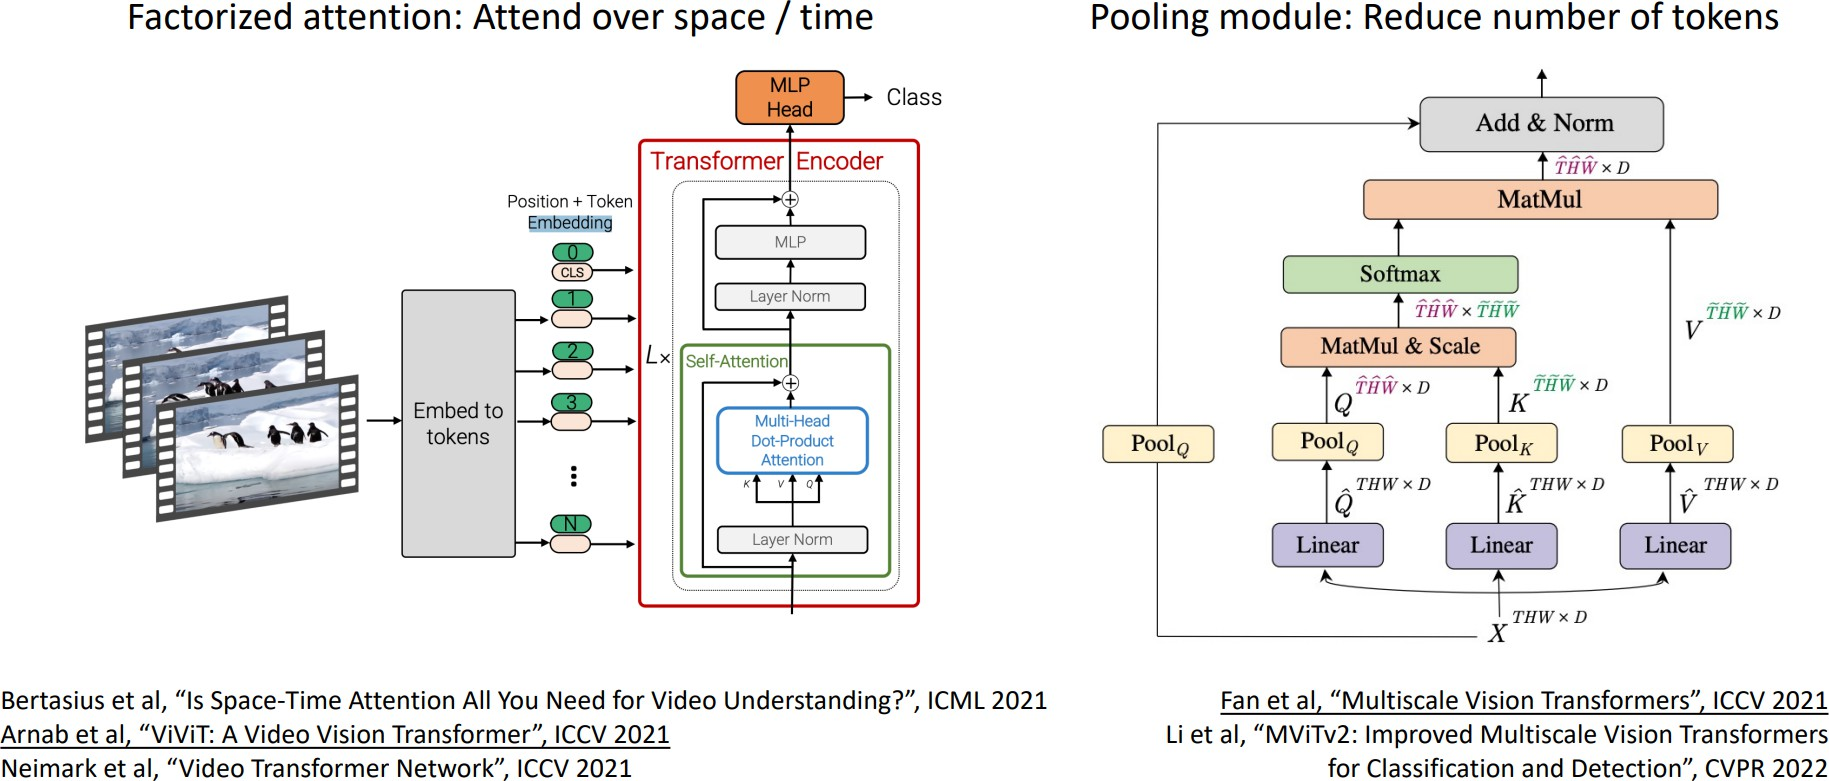
\includegraphics[width=1\textwidth,height=0.9\textheight,keepaspectratio]{images/video/slide_38_1_img.jpg}
    \end{figure}
\framebreak
    \begin{figure}
        \centering
        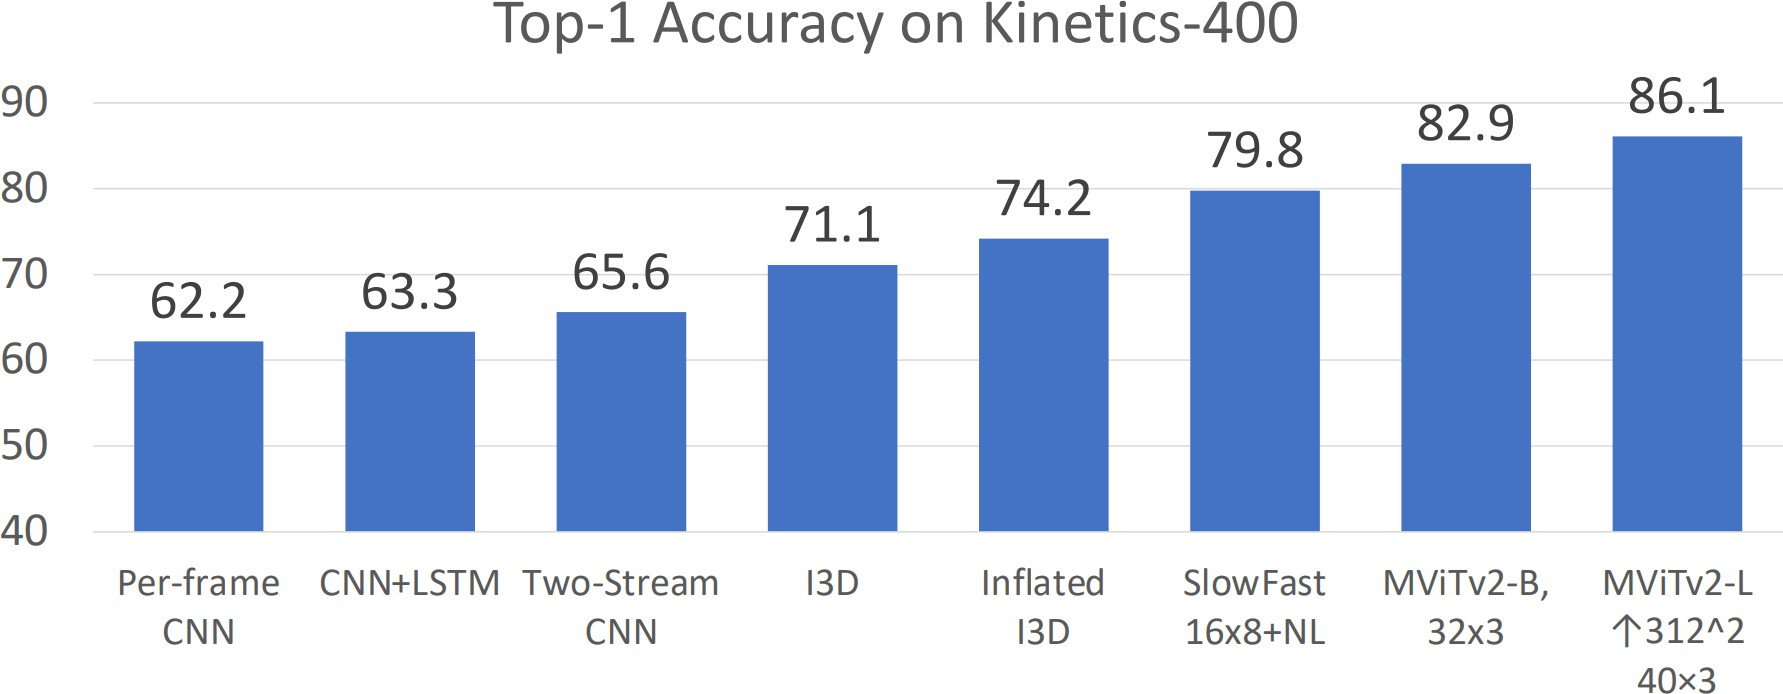
\includegraphics[width=1\textwidth,height=0.9\textheight,keepaspectratio]{images/video/slide_39_1_img.jpg}
    \end{figure}
\end{frame}